\subsection{Problem 6.5. Designing Bus Routes}

\paragraph{}
\begin{quote}
GTC has a research wing set up in the city marked A in Figure \ref{figure6-23}. The personnel for this wing come from the neighboring villages, marked from B through P in the same figure. The figure also schematically provides the road network between these villages, with the length of the road segment between a pair of villages (in kilometers) marked on the line joining the two. For example, villages B and C are connected by a road 1.0 kilometer long.
GTC wants to make use of a bus service to pick up all the personnel from their villages at the start of the day, and drop them back after work. It is negotiating a contract with a local bus service company BSC. The bus service company has given GTC two options.
In the first option, BSC provides GTC with a long distance bus, which starts at A and with which GTC can pick up all its personnel in one round trip and deposit them to its research wing at A. The cost of hiring the bus is \texteuro 2000 per month, and BSC will charge \texteuro 7.50 per kilometer traveled by the bus in each month.
In the second option, BSC will provide GTC with two minibuses. These minibuses can travel up to 10 kilometers in one trip. Using these buses, GTC has to plan two round trips to transport all its personnel to and from the research wing. The cost of hiring each minibus is \texteuro 1050 per month and BSC will charge as usual \texteuro 7.00 per kilometer traveled by the bus in each month.
On an average, GTC works 20 days in a month.
\end{quote}

\begin{figure}[H]
	\centering
	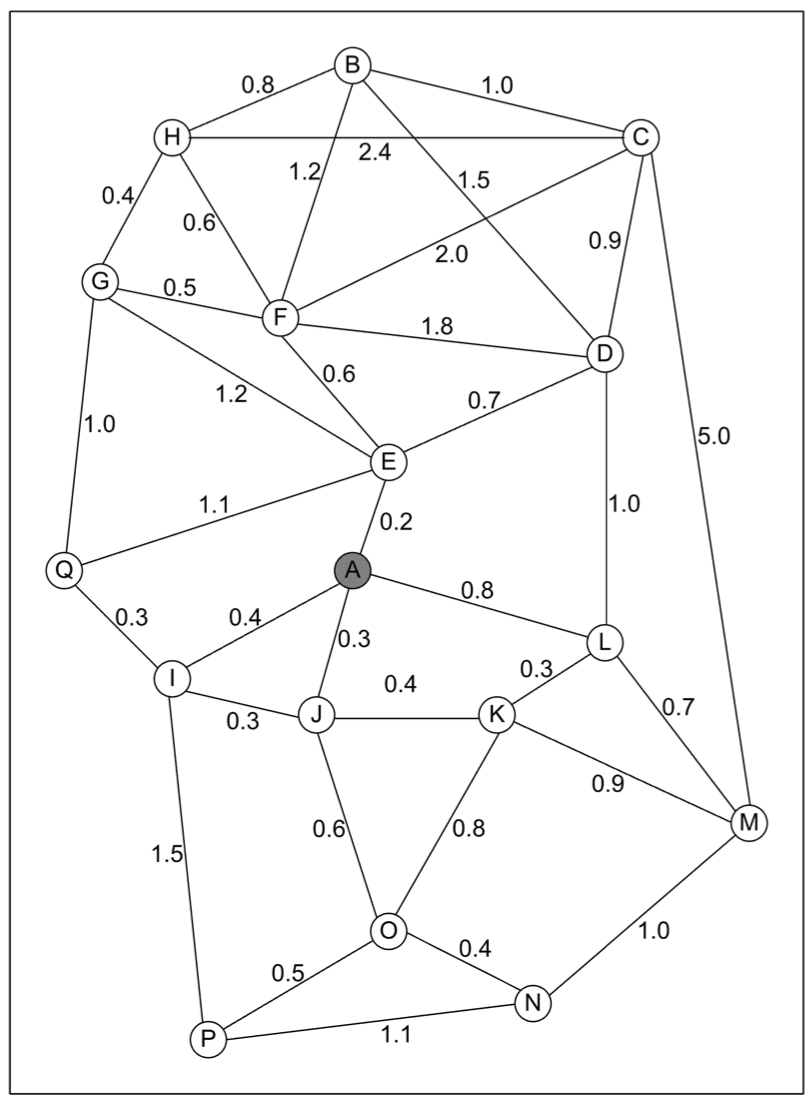
\includegraphics[scale=1]{./img/figure6-23.png}
	\caption{Distance map for the region}
	\label{figure6-23}
\end{figure}

\paragraph{}
We consider a weighted graph with 17 vertices and 35 edges, obtained in a straightforward way from figure \ref{figure6-23}. The vertices correspond to villages and city, the edges correspond to road segments, the weights of the edges correspond to road segments lengths. Paths in this graph correspond to routes. Cycles correspond to round trips. We'll call this graph the source graph. We also consider a complete graph of shortest distances between all pairs of vertices of the graph. We'll call this graph the closure graph. Each path or cycle in closure graph corresponds to a path or cycle in source graph, which can be obtained by replacing each edge with the shortest path between its endpoints.

\paragraph{}
We used Floyd-Warshall algorithm for finding the closure graph.

\paragraph{(a)}
\begin{quote}
GTC wants to figure out the approximate cost per month of operating under the first option. Starting at city A, use the nearest insertion heuristic to come up with a feasible route and the cost of operating this route. What do you observe?
\end{quote}

\paragraph{}
In source graph we need to find the shortest cycle that goes through each vertex at least once. It is equivalent to finding the shortest cycle in closure graph that goes through each vertex exactly once (i.e. solving TSP). It's quite obviuos, but let's prove it just in case. Consider the sought-for shortest cycle in source graph. If we remove from this path all vertices that were already visited earlier in this path, we obtain a cycle in closure graph that has the same total weight. Similarly, the shortest cycle in closure graph corresponds to a cycle with the same total weight in the source graph. This means that these weights are equal, and optimal cycles in source and closure graphs correspond to each other.

\paragraph{}
We used the nearest insertion heuristic on closure graph. The resulting route (translated back to source graph) is $ A \rightarrow I \rightarrow Q \rightarrow I \rightarrow J \rightarrow O \rightarrow P \rightarrow O \rightarrow N \rightarrow O \rightarrow N \rightarrow M \rightarrow L \rightarrow K \rightarrow J \rightarrow A \rightarrow E \rightarrow D \rightarrow C \rightarrow B \rightarrow H \rightarrow G \rightarrow F \rightarrow E \rightarrow A $. This monthly cost is \texteuro 5630.

\paragraph{}
The part $ O \rightarrow N \rightarrow O \rightarrow N $ looks suspicious. How could our heuristic produce such locally inefficient cycle? Let's take a look at the corresponding cycle in closure graph: $ A \rightarrow Q \rightarrow I \rightarrow P \rightarrow N \rightarrow O \rightarrow M \rightarrow L \rightarrow K \rightarrow J \rightarrow D \rightarrow C \rightarrow B \rightarrow H \rightarrow G \rightarrow F \rightarrow E \rightarrow A $. This cycle looks ok, and the part $ P \rightarrow N \rightarrow O \rightarrow M $ produces the weird part of the route. This production appears to be correct as well. It turns out that the expansion of the cycle in closure graph to route in source graph just made the unoptimality of the solution more obvious.

\paragraph{(b)}
\begin{quote}
Find the lowest cost that GTC would have to pay to operate under the first option.
\end{quote}

\paragraph{}
We used dynamic programming to solve the TSP in closure graph in $O(2^n n^2)$, where $n$ is the number of vertices. The resulting cheapest route is $ A \rightarrow I \rightarrow Q \rightarrow I \rightarrow J \rightarrow O \rightarrow P \rightarrow O \rightarrow N \rightarrow M \rightarrow K \rightarrow L \rightarrow D \rightarrow C \rightarrow B \rightarrow H \rightarrow G \rightarrow F \rightarrow E \rightarrow A $. The monthly cost is \texteuro 5270.

\paragraph{(c)}
\begin{quote}
Find by inspection, two routes that the GTC could operate under if they chose the second option. What is the rationale behind your choice? What is the cost of
operating these two routes?
\end{quote}

\paragraph{}
We chose the routes $ A \rightarrow I \rightarrow Q \rightarrow G \rightarrow H \rightarrow F \rightarrow B \rightarrow C \rightarrow D \rightarrow E \rightarrow A $ of monthly cost \texteuro 2926 and $ A \rightarrow L \rightarrow K \rightarrow M \rightarrow N \rightarrow P \rightarrow O \rightarrow J \rightarrow A $ of monthly cost \texteuro 2590. The total monthly cost is \texteuro 5516. When constructing the route we tried to split the vertices evenly between routes and to take locally shorter edges.

\paragraph{(d)}
\begin{quote}
Using these two routes as a starting solution, and transforming the problem into
a TSP, see if you can apply the 2-opt heuristic to improve the routes obtained in
part (c).
\end{quote}

\paragraph{}
We spread the vertices of closure graph in two sets, corresponding to vertices of the two cycles. Vertex A is included in both sets. In each set our cycle found by inspection gives a plausible traveling salesman cycle. We apply 2-opt heuristic to these cycles independenty. The resulting routes are $ A \rightarrow I \rightarrow Q \rightarrow G \rightarrow F \rightarrow H \rightarrow B \rightarrow C \rightarrow D \rightarrow E \rightarrow A $ with cost \texteuro 2842 and $ A \rightarrow J \rightarrow K \rightarrow L \rightarrow M \rightarrow N \rightarrow O \rightarrow P \rightarrow O \rightarrow J \rightarrow A $ with cost \texteuro 2450. The total cost is \texteuro 5292.

\paragraph{(e)}
\begin{quote}
What is the lowest cost that GTC would have to pay to operate under the second
option. How different is it from your answer in part (d)? Based on your result
should GTC use the first option or the second one?
\end{quote}

\paragraph{}
The problem can be reformulated as follows. We need to divide the vertices of closure graph in two disjoint subgraphs (with the exception that vertex A must be in both subgraphs) such that the sum of TSP cycle lengths in the two subgraphs is minimal. To do this we first use the same dynamic programming as in (b) to find for each set of vertices the minimum length of TSP cycle spanning these vertices. Then we just iterate over all sets of vertices and find the minimum sum of corresponding two TSP lengths. The overall complexity is $O(2^n n^2)$.

\paragraph{}
The optimal routes are $ A \rightarrow E \rightarrow F \rightarrow G \rightarrow H \rightarrow B \rightarrow C \rightarrow D \rightarrow E \rightarrow A $ of cost \texteuro 2534 and $ A \rightarrow J \rightarrow O \rightarrow P \rightarrow O \rightarrow N \rightarrow M \rightarrow L \rightarrow K \rightarrow J \rightarrow I \rightarrow Q \rightarrow I \rightarrow A $ of cost \texteuro 2730. The total monthly cost is thus \texteuro 5264, which is slightly less than the optimal cost under the first option. GTC should use the second option.

\paragraph{(f)}
\begin{quote}
GTC argues that the requirement of round trips is constraining the routes cho-
sen under the second option Can you provide an example in support of GTC’s argument?
\end{quote}

\paragraph{}
Instead of making the same round trip twice a day (to take everyone from home to work and back), the buses can do one trip from some village to the city (to take everyone from home to work) and one trip from the city to the same village (to take everyone home). This problem is similar to the one in (e), but instead of two TSP cycles we need two TSP paths from vertex A to any other vertex. We used the same algorithm, but instead of precalculating the lengths of optimal TSP round trips we precalculated the lengths of optimal TSP paths from vertex A to any vertex.

\paragraph{}
The optimal paths are $ A \rightarrow E \rightarrow F \rightarrow G \rightarrow H \rightarrow B \rightarrow C \rightarrow D $ of cost \texteuro 2282 and $ A \rightarrow I \rightarrow Q \rightarrow I \rightarrow J \rightarrow K \rightarrow L \rightarrow M \rightarrow N \rightarrow O \rightarrow P $ of cost \texteuro 2338. The total cost is \texteuro 4620, which is indeed considerably less than in (e).
